%Version en ligne
\documentclass[12pt,a4paper]{report}
%Version imprimable
%\documentclass[12pt,a4paper,twoside,openright]{report}

% ***** relative path from this file's folder to the template folder *****
\newcommand{\baserelpath}{../../../..} % FIXME

% ***** preamble (needed, do not remove or modify) *****
\newcommand{\baserelTPpath}{\baserelpath/templates/tp}
% ************************
% * fichier de préambule *
% ************************

% ***** extensions *****
\usepackage[T1]{fontenc}	% Caractères accentués et césure
\usepackage[utf8x]{inputenc}	% Choix de l'encodage
\usepackage{graphicx}		% Paquage pour l'insertion d'images
\usepackage{wrapfig}		% Figures flottantes
\usepackage[french]{babel}	% Support Français
\usepackage{eurosym}		% Signe € qui s'adapte en fonction de la police
\usepackage{fancyhdr}		% En-tête de pages personalisés
\usepackage{color}		% Un peu de couleurs
\usepackage{array}		% Faire des beaux tableaux
% Liens cliquables dans le document
\usepackage[colorlinks=true,linkcolor=black,urlcolor=blue,%
pdftitle={Workshop GConfs},pdfauthor={GConfs}]{hyperref}
\usepackage{amsmath}		% Formules matématiques
\usepackage{listings}           % Mise en forme de code source

% Changement des polices du document
\usepackage{palatino}
\usepackage[sc]{mathpazo}
\linespread{1.05}


% ***** césures particulières *****

\hyphenation{}

% ***** filigrane *****
%\usepackage{eso-pic,rotating}
%\AddToShipoutPicture{%
%\unitlength 1cm
%\put(11,15){%
%\begin{rotate}{45}
%\makebox(0,0){\color{lightgray}\scalebox{3.5}{\Huge BROUILLON}}
%\end{rotate}}
%}

% ***** couleurs perso *****

\definecolor{lightgray}{RGB}{240,240,240}

\definecolor{vert}{RGB}{0,176,80}
\definecolor{verta}{RGB}{79,97,40}
\definecolor{vertb}{RGB}{195,214,155}
\definecolor{vertc}{RGB}{235,241,221}
\definecolor{bleua}{RGB}{31,73,125}
\definecolor{bleub}{RGB}{219,229,241}
\definecolor{rougea}{RGB}{192,80,77}
\definecolor{rougeb}{RGB}{242,220,219}

\definecolor{brown}{RGB}{128,0,0}
\definecolor{blue}{RGB}{0,0,255}
\definecolor{green}{RGB}{0,128,0}
\definecolor{seagreen}{RGB}{69,158,181}


% ***** paramètre de la coloration syntaxique *****
\lstset{language=[Sharp]C,basicstyle=\ttfamily\footnotesize,%
stringstyle=\ttfamily\color{brown},commentstyle=\color{green},%
%numberstyle=\footnotesize,stepnumber=1,numbersep=7pt,%
backgroundcolor=\color{vertc},frame=single,tabsize=2,breaklines=true,%
breakatwhitespace=false,%
classoffset=0,% Mots clés non reconnus
morekeywords={},keywordstyle=\color{blue},%
classoffset=1,% Noms de classes
morekeywords={Console},keywordstyle=\color{seagreen},%
classoffset=0
}

% ***** commandes personnelles *****

\newcommand{\helpbox}[3][bleu]{\vspace{1em}\fcolorbox{#1a}{#1b}{\parbox{.92%
\linewidth}{\hspace{5pt}\textbf{#2~:} #3}}\vspace{0.75em}}
\newcommand{\warnbox}[3][rouge]{\vspace{1em}\fcolorbox{#1a}{#1b}{\parbox{.92%
\linewidth}{\hspace{5pt}\textbf{#2~:} #3}}\vspace{0.75em}}
\newcommand{\tp}{workshop}
\newcommand{\Tp}{Workshop}
\newcommand{\svn}{\textsc{svn}}
\makeatletter
\renewcommand{\chapter}{\clearpage%
     \@startsection{chapter}{1}{-0.75em}{\baselineskip}%
     {0.5\baselineskip}{\LARGE\textbf}}
\makeatother
\renewcommand{\thechapter}{\Roman{chapter}}
\renewcommand{\thesection}{\arabic{section}}

% ***** en-têtes et pieds de pages *****
\pagestyle{fancyplain}
	\lhead[\emph{\nouppercase{\leftmark}}]{\emph{\textit{\Tp{} TP\_title (in preambule.tex)}}}
	\chead{} 
	\rhead[\emph{\textit{\Tp{} TP\_title (in preambule.tex)}}]{\emph{\nouppercase{\leftmark}}}
	\lfoot[]{\small{\textit{GConfs 2011}}}
	\rfoot[\small{\textit{GConfs 2011}}]{}


% ***** for code listings *****
\lstsetparams{Sharp}{C}{}{Value,Convert,Exp,Cst}

% ***** workshop title (used as pages' head) *****
\newcommand{\workshoptitle}{CAS et évaluation d'expressions} % FIXME

% ***** page heading and foot *****
\headfootparams{\workshoptitle}

% ***** to display a "BROUILLON" in all pages *****
%\makefiligrane

\newcommand{\cas}{\textsc{CAS}}
\newcommand{\npi}{\textsc{npi}}

\begin{document}

\title{
  \vspace{1cm}
  \textbf{\Huge{\Tp{} \workshoptitle}}\\
  %\vspace{1cm}
  %\includegraphics[scale=0.75]{images/logo.png}
}
\author{
  \Large{Raphaël \textit{Black Chatou} \textsc{Boissel} ({\ttfamily boisse\_r})}\\\\
}

\date{
  \vspace{1cm}
  % GConfs logo
  \includegraphics[scale=0.5]{\baserelTPpath/images/gconfs.png}\\
  \vspace{0.5cm}
  Day xx Month 201x
}
\maketitle
\newpage
\tableofcontents
\newpage

% beginning of document
\section{Présentation du workshop}

\subsection{Définition du \textsc{cas}}

Le \cas{} (Computer Algebra System ou système de calcul formel en français), est un système qui a pour objectif de travailler sur des expressions mathématiques qui contiennent par exemple des inconnues ($x$, $y$, \ldots) ou des symboles ($\pi$, $e$, \ldots). Le \cas{} peut faire des opérations telles que la dérivé d'une expression ou la recherche des solutions d'une équation.\\

Exemple d'expression sur laquelle un \cas{} peut travailler~:
$$5*\pi+2*x$$

\subsection{Définition de l'évaluation}

Contrairement au \cas{} l'évaluation de l'expression va consister à travailler sur des quantités connues et finies. On utilisera alors des variables dont la valeur a été préalablement définie et les constantes telles que $\pi$, $e$, \ldots{} seront approximées. Le but de l'évaluation est de fournir une valeur.

\subsection{Objectif}

L'objectif de ce workshop est de créer en C\# un petit logiciel qui puisse à la fois faire divers traitements sur une expression comme la dérivée, ou la simplification et qui soit également capable de faire l'évaluation de cette expression à condition qu'on spécifie les valeurs des variables se trouvant dans l'expression.



\section{Créer l'interface utilisateur}

\subsection{Création d'une application Windows Forms}

Lorsque vous créez un nouveau projet dans \textit{Visual Studio} vous vous trouvez face à une multitude de choix. Dans notre cas nous allons utiliser une \textit{Application Windows Forms} que nous nommerons \textit{CAS}. Une fois l'application créée une fenêtre nommée \texttt{form1} apparaît à l'écran. À l'aide de la boite à outils (généralement située sur le côté de l'écran) nous allons insérer les composants suivants~:

\begin{itemize}
	\item un champ de texte (\texttt{TextBox}) qui nous servira à rentrer les lignes de calculs à traiter,
	\item un bouton qui déclenchera l'évaluation de l'expression,
	\item un bouton qui simplifiera l'expression,
	\item un bouton qui dérivera l'expression,
	\item une liste de choix (\texttt{ListBox}) qui contiendra l'historique de toutes les opérations effectuées,
	\item un bouton qui permettra d'effacer l'historique.
\end{itemize}
\vspace{1em}
Une fois tous ces composants ajoutés, notre interface devrait ressembler à ceci~:

\begin{figure}[ht]
	\begin{center}
		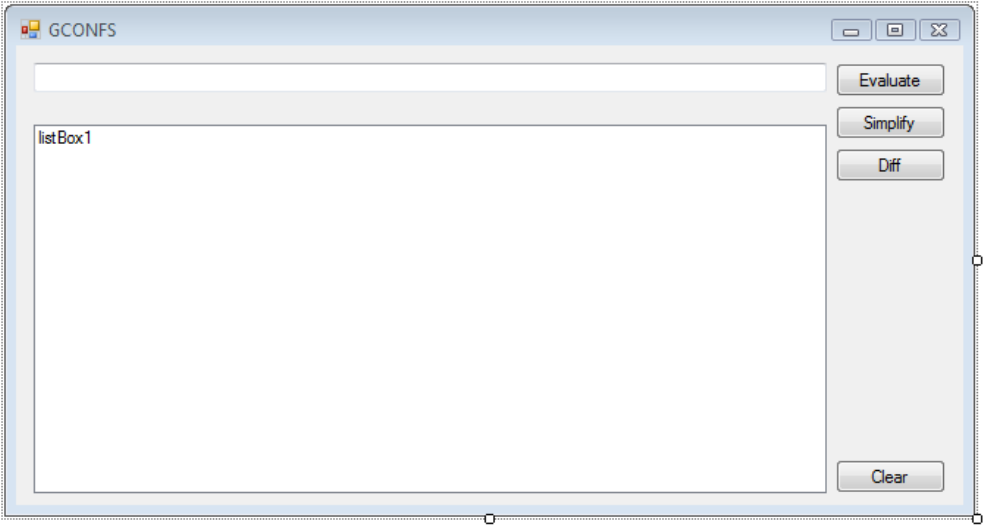
\includegraphics[scale=0.5]{form1}
		\caption{Exemple d'interface}
		\label{fig:form1}
	\end{center}
\end{figure}

La disposition est bien entendu laissée à votre convenance~: soyez créatif~!

\subsection{La fonction d'effacement}

La première fonction que nous allons coder est la fonction qui permet d'effacer l'historique, c'est-à-dire celle qui permet de vider la liste de choix, lorsque l'on appuie sur \textit{Clear}.

\helpbox{Aide}{pour créer une fonction qui est appelée au moment où on clique sur un bouton, double-cliquez simplement sur le bouton en question.}



\section{Les valeurs}

\subsection{La création de la classe \texttt{Value}}

Nous allons commencer par créer une classe \texttt{Value}. Cette classe représentera une valeur constante de la forme~:

$$a+b*\pi+c*e$$

Classe dans laquelle nous ajouterons donc trois valeurs flottantes $a$, $b$, $c$. On demande ici uniquement la création de la classe~: les méthodes qui vont modifier les valeurs de ces variables seront écrites plus tard.

\helpbox{Note}{cette représentation va nous permettre par exemple d'effectuer des opérations telles que $2\pi+\pi$ sans perte de précision.}

\subsection{Les opérations}

C\# nous donne la possibilité de définir nos propres opérateurs ($+$, $-$, $*$, $/$,~\ldots) sur des types que nous avons nous-même créés. C'est ce que nous allons faire avec \texttt{Value}. En effet, il serait agréable de pouvoir utiliser directement les opérateurs $+-*/$ sur nos valeurs plutôt que de faire appel à des fonction comme \texttt{Add}, \texttt{Sub}, \ldots qui alourdiraient vite le code.

La syntaxe est la suivante~:

\begin{lstlisting}
public static Value operator +(Value A, Value B)
{
	Value C = new Value();
	// Fix Me;
	return C;
}
\end{lstlisting}

\helpbox{Note}{un opérateur doit obligatoirement être déclaré {\ttfamily public static}.}

Nous allons donc coder les opérateurs $+$ , $-$, $*$ et $/$ en considérant que si l'un des deux membres de l'opération est un flottant le résultat sera sous la forme d'un flottant.

\subsection{Les conversions implicites}

Parfois il serait plus agréable de pouvoir utiliser un \texttt{int} ou un \texttt{float} en tant que \texttt{Value} et inversement. Pour cela C\# dispose des opérateurs de conversions implicites~: c'est-à-dire que c'est le compilateur qui décidera quand est-ce-qu'il est nécessaire d'utiliser un \texttt{int} ou un \texttt{float} ou bien une \texttt{Value}.

La syntaxe est la suivante~:

\begin{lstlisting}
public static implicit operator Value(int A)
{
	Value C = new Value();
	// Fix Me;
	return C;
}
\end{lstlisting}

\helpbox{Note}{l'extrait de code ci-dessus montre comment écrire une conversion implicite d'un {\ttfamily int} vers une {\ttfamily Value}.}

Nous allons donc écrire les conversions suivantes~:
\begin{itemize}
	\item {\ttfamily int} $\rightarrow$ {\ttfamily Value}
	\item {\ttfamily float} $\rightarrow$ {\ttfamily Value}
	\item {\ttfamily Value} $\rightarrow$ {\ttfamily float}
\end{itemize}

\subsection{Chaînes de caractères et {\ttfamily Value}}

\subsubsection{Une {\ttfamily Value} vers une chaîne}

On se propose d'écrire la fonction \texttt{ToString()} qui retourne la chaîne de caractères correspondante à la valeur. Voici le prototype de la fonction~:

\begin{lstlisting}
public override string ToString()
{
	// Fix Me;
}
\end{lstlisting}

\helpbox{Note}{le mot-clé {\ttfamily override} vient du fait qu'il existe une méthode {\ttfamily ToString} par défaut dans chaque classe.}

\subsubsection{Une chaîne vers une {\ttfamily Value}}

On se propose d'écrire la fonction \texttt{FromString()} qui retourne la valeur correspondante à une chaîne de caractères.

Afin de simplifier la fonction et parce que les autres cas sont inutiles, nous ne considèrerons que les chaînes de caractères de la forme suivante~:

\begin{itemize}
	\item "$10$", "$10.0$" , "$11.97$", "$-11.97$", \ldots
	\item "$10\,\pi$", "$10.0\,\pi$", "$11.97\,\pi$", "$-11.97\,\pi$", \ldots
	\item "$10\, e$", "$10.0\, e$", "$11.97\, e$", "$-11.97\, e$", \ldots
\end{itemize}

On considérera également qu'il y a toujours une espace entre le nombre et $\pi$ ou $e$.\\

Les opérations suivantes sur les chaînes de caractères pourront être utilisées~:

\begin{lstlisting}
string number = "10.0";
number = number.Replace(".", ",");
	// number contient maintenant "10,0"
float a = Convert.ToSingle("10,65");
	// le nombre doit contenir une , et non un . pour que ToSingle fonctionne
\end{lstlisting}

Voici le prototype de la fonction~:

\begin{lstlisting}
public static Value FromString(string str)
{
	// Fix Me;
}
\end{lstlisting}

\helpbox{Note}{La méthode est statique car elle retourne une nouvelle {\ttfamily Value}. Elle n'a donc pas besoin de dépendre d'une {\ttfamily Value} déjà existante (d'une \textit{instance} de \texttt{Value}). On aurait également pu écrire cela comme un constructeur.}

\subsection{Est-ce que c'est zéro~?}

Il faut maintenant créer la méthode \texttt{IsNull} qui retourne vraie seulement si la \texttt{Value} vaut 0 c'est-à-dire si $a=b=c=0$ (on laissera de côté les cas pathologiques de la forme $a=0$ $b=-e$ et $c=\pi$).\\\\\\

Voici le prototype de la fonction~:

\begin{lstlisting}
public static bool IsNull()
{
	// Fix Me;
}
\end{lstlisting}




\section{Les expressions}

\subsection{La classe abstraite {\ttfamily Exp}}

Nous allons créer la classe abstraite \texttt{Exp} qui va définir les
méthodes qui devront être présentes dans chacune des classes qui vont
hériter de \texttt{Exp}. Cette classe abstraite va se contenter de
définir les prototypes des méthodes et non les implémenter. Afin
d'éviter tout problème lors de la réalisation de cette classe le code
basique de la classe est disponible ci-dessous~:

\begin{lstlisting}
abstract class Exp
{
	public abstract Exp Simplify();
	public abstract Exp Diff(string Var);
	public abstract Value Evaluate(Dictionary<string, Value> Variables);
	public abstract Value ToValue();
	public abstract bool IsNull();
	public abstract bool IsConst();
	public virtual new string ToString(){return "";}
}
\end{lstlisting}

Par la suite nous allons modifier cette classe mais pour le moment,
nous pouvons continuer en la laissant en l'état.

\subsection{L'expression constante}

Commençons par coder une expression assez particulière, l'expression constante.

Pour déclarer une classe qui hérite d'une autre classe la syntaxe est la suivante~:

\begin{lstlisting}
class Cst : Exp
{
}
\end{lstlisting}

Toute classe qui hérite d'une classe abstraite doit impérativement
redéfinir les méthodes marquées comme \texttt{abstract}, déclarées
dans la classe abstraite dont il hérite. Dans notre cas \texttt{Cst}
va devoir redéfinir \texttt{Simplify}, \texttt{Diff},
\texttt{Evaluate}, \texttt{ToValue}, \texttt{IsNull},
\texttt{IsConst}, \texttt{ToString} (même si cette méthode est marquée
comme \texttt{virtual} et non comme \texttt{abstract}, nous allons
quand même la redéfinir). Pour redéfinir une méthode dans une classe
il faut utiliser la syntaxe ci-dessous~:

\begin{lstlisting}
public override bool IsConst()
{
	// Fix Me;
}
\end{lstlisting}

Maintenant que nous savons comment faire nous allons le
faire. L'expression constante est une expression qui est construite
avec une valeur. Il est donc nécessaire d'écrire un constructeur dont
le prototype est le suivant~:

\begin{lstlisting}
public Cst(Value value)
{
	// Fix Me;
}
\end{lstlisting}

\helpbox{Note}{vous devez définir la/les différentes variable(s) nécessaire(s) vous-même pour que ce constructeur puisse fonctionner.}

La particularité de la classe constante est que quelque soit
l'ensemble de variables passé en paramètre, \texttt{Evaluate} renverra
toujours la valeur avec laquelle la classe a été construite. La dérivé
renverra toujours la constante construite avec la valeur nulle
(\texttt{new
Cst(0)}). \texttt{IsNull} testera si la valeur est nulle,
\texttt{IsConst} renverra toujours vrai, \texttt{ToValue} retournera
la valeur avec laquelle la classe a été initialisée et
\texttt{ToString} retournera la chaîne de caractères correspondant à
la valeur avec laquelle la chaîne a été initialisée.

Implémentons donc ces méthodes.\\

\texttt{Symplify} est une commande qui renvoie l'expression simplifiée
mais comme dans le cas d'une constante il n'y a rien à simplifier,
nous renverrons simplement une nouvelle constante initialisée avec la
même valeur que la première.

\subsection{L'expression variable}

La structure de l'expression variable reprend celle de la constante~:

\begin{lstlisting}
class Var : Exp
{
}
\end{lstlisting}

Nous commencerons donc par écrire le constructeur de l'expression variable qui prend en paramètre une \texttt{string} qui représentera le nom de la variable~:

\begin{lstlisting}
public Var(string value)
{
	// Fix Me;
}
\end{lstlisting}

\helpbox{Note}{vous devez définir la/les différentes variable(s) nécessaire(s) vous même pour que ce constructeur puisse fonctionner.}

Il devrait être assez facile maintenant d'implémenter les méthodes
\texttt{Diff}, \texttt{ToValue}, \texttt{IsNull}, \texttt{IsConst},
\texttt{ToString}. On considérera que \texttt{IsNull()} ne peut jamais
être vraie et que \texttt{ToValue} renvoie \texttt{null}
(\texttt{ToValue} n'existe que s'il y a possibilité de transformer
l'expression en valeur or ce n'est pas le cas ici).\\

Intéressons nous maintenant à \texttt{Evaluate}. Pour accéder à un
dictionnaire, la syntaxe est la même que pour accéder à un tableau. En
effet, pour récupérer la valeur de la variable \texttt{toto} dans le
dictionnaire de variables, en supposant qu'elle existe, il suffit de
faire \texttt{Variables[toto]} et nous obtiendrons sa valeur. En
sachant cela nous pouvons donc coder la fonction \texttt{Evaluate}
pour les expressions variables.\\

Une fois de plus pour \texttt{Symplify} il n'y a rien à simplifier,
nous renverrons simplement une nouvelle expression variable
initialisée avec la même valeur que la première.

\subsection{Les autres expressions}

Après avoir codé les deux expressions particulières nous allons
maintenant pouvoir travailler sur des expressions plus
conventionnelles. Nous allons commencer par coder l'addition
(\texttt{Add}), la soustraction (\texttt{Sub}), la division
(\texttt{Div}) et la multiplication (\texttt{Mul}). Vous pouvez bien
sûr rajouter par la suite autant d'expression qu'il vous plaira~:
$\cos$ et $\sin$ par exemple.\\

Toutes ces expressions ont un constructeur similaire qui prend en
paramètre deux expressions (\texttt{A} et \texttt{B}) qui sont
respectivement la partie gauche et la partie droite de l'opération~:

\begin{lstlisting}
public Add(Exp A, Exp B)
{
	// Fix Me;
}
\end{lstlisting}

Ainsi pour déclarer $Toto=5+2$ nous déclarerons~: \texttt{toto = new Add(new Cst(5), new Cst(2))}.\\

Nous pouvons à présent coder toutes les opérations nécessaires pour que ces expressions fonctionnent correctement.

\helpbox{Note}{Soignez particulièrement votre fonction de simplification pour chaque expression~; c'est elle qui fera la force de votre \cas.}


\section{Créer une expression à partir d'une {\ttfamily string}}

\subsection{Lecture d'une chaîne en NPI (Notation Polonaise Inverse)}

Vous connaissez sans doute le principe de la notation polonaise inverse. Pour rappel, $5 + 8 * 6$ s'écrit en \npi{} $8\,6\,*\,5\,+$.

À vous de trouver un algorithme (en utilisant une pile de \texttt{string}~: \texttt{Stack<string>} en C\#) qui permet de transformer une chaîne en \npi{} vers une expression.

\helpbox{Note}{On pourra utiliser un {\ttfamily switch} \ldots {\ttfamily case}}

\subsection{Lecture d'une chaîne en notation infixe}

La notation infixe est la notation que nous utilisons tous les jours.
Par exemple~:
$$(5+x)*10*(\pi+10)$$

La prise en charge de ce genre de notation est une étape plutôt délicate. C'est pourquoi nous allons procéder en deux temps. Dans un premier temps nous allons convertir la chaîne en notation infixe vers une chaîne en \npi{} puis nous utiliserons la fonction précédemment écrite pour en extraire une expression.\\

Un des algorithmes qui permet de passer d'une notation infixe à une notation en \npi{} s'appelle Shunting-yard algorithm (littéralement algorithme de la voie de garage). Le nom de cet algorithme vient de la façon dont on procède pour créer la chaîne en \npi.\\

Voici une version simplifiée de son fonctionnement~:

On utilisera une pile de \texttt{string} (\texttt{Stack<string>} en C\#) pour la voie de garage et une \texttt{string} pour la sortie.

\begin{itemize}
	\item L'élément est $($~: on empile $($
	\item L'élément est $)$~: on dépile et on met les éléments dépilés dans la sortie jusqu'à trouver l'élément $($. L'élément $($ ne sera pas ajouté à la sortie.
	\item L'élément est \textbf{un nombre ou une variable}~: on le met directement dans la sortie
	\item L'élément est \textbf{un opérateur \textit{opp1}}~:
	\begin{enumerate}
		\item Tant qu'il y a un opérateur \textit{opp2} sur le sommet de la pile et que la priorité de \textit{opp2} est supérieure ou égale à la priorité de \textit{opp1}, on dépile \textit{opp2} et on le met dans la sortie.
		\item On met \textit{opp1} au sommet de la pile.
	\end{enumerate}
\end{itemize}

Quand il n'y a plus d'éléments on dépile les éléments de la pile jusqu'à ce que la pile soit vide.

\warnbox{Attention}{cet algorithme ne marche que si tous les opérateurs sont associatifs à gauche. Voir le véritable Shunting-yard algorithm pour les autres cas.}

\section{Finir l'interface}

Maintenant que notre \cas{} est capable de plein de choses, il faut finir l'interface afin de permettre à l'utilisateur de rentrer une expression puis d'effectuer tout un tas d'opérations dessus. Pour cette dernière étape vous êtes totalement libre~!

% end of document
\end{document}
